\chapter{System design}

In this chapter, component selection and design is described. 

\section{Space segment}
Space segment is a part of the satellite communication system that resides on the satellite itself. It is divided into two main parts: communication subsystem (COMM) and antennas (ANTs) connected with two coaxial cables.

Space segment is critical in system operation and reliability - there is no possibility to carry out any repairs. It is exposed to the space environment - thermal cycling, cosmic radiation and vacuum.

Because of the mentioned requirements it was decided to choose commercially available and flight-proven Cubesat components to increase the reliability of the system.

\subsection{Frequency band selection}
Data throughput requirements and communication session scheme were described in the \ref{introduction} chapter, but it summarizes to about \SI{1}{\kilo\byte / \second}.

As mentioned in section \ref{???} the most common radio bands used in Cubesat designs are VHF, UHF and S-band. S-band is usually used when high data rate (~\SI{10}{\mega\bits / \second}) are necessary. Typical designs for low-rate data link are full-duplex combo or simplex VHF/UHF radio.

PW-Sat1 (first polish satellite, built on Warsaw University of Technology) - (link)??? used full-duplex VHF-downlink and UHF-uplink radio. During its mission, uplink stability was an issue. The cause was narrowed down to very high level of noise and interference in the UHF band on the orbit, which probably is caused by over-the-horizon radars. Therefore, UHF-uplink was discarded.

Concluding, the selected band for operation were either simplex VHF or VHF-up, UHF-down full-duplex.

\subsection{Communication subsystem}
Communication subsystem of the satellite is responsible of transmitting and receiving radio signals, modulating/demodulating them and providing data link for the On Board Computer. It has to be compatible with selected mechanical configuration, available data interfaces and the antennas to be installed.

Cubesat standard, with which PW-Sat2 is compliant, defines PC/104 connector, which is the main data bus for all satellite subsystems. Radio should use \iic bus to send and receive data from the on-board computer.

When the subsystem was ordered, the choice of available products was very limited, and the only radio which was compliant with above mentioned requirements was \texttt{ISIS VHF uplink/UHF downlink Full Duplex Transceiver}. Its view and block diagram is shown in the figure \ref{ISIS_TRXvU}

\begin{figure*}
   \centering
\begin{tabular}{cc}
        \includegraphics[width=0.4\paperwidth]{img/2/ISIS-radio-UHF-VHF-min.png}
    & 
        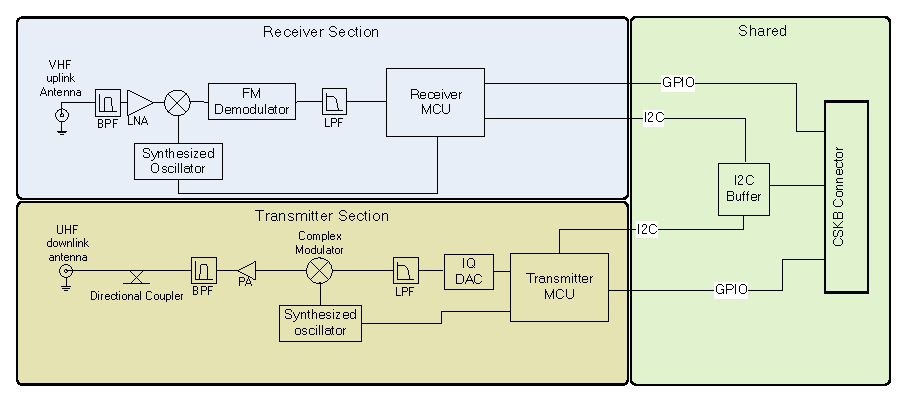
\includegraphics[width=0.3\paperwidth]{img/2/ISIS_TRXvU_block_diagram.eps}
\end{tabular}
\label{ISIS_TRXvU}
\caption{ISIS VHF uplink/UHF downlink Full Duplex Transceiver. Source: \cite{???}}
%%% https://www.isispace.nl/product/isis-uhf-downlink-vhf-uplink-full-duplex-transceiver/
\end{figure*}

Basic characteristics:

\begin{tabular}{c|c}
     \textbf{downlink} & \textbf{uplink} \\ \hline
     \multicolumn{2}{c}{dual-\iic communication standard} \\
     \multicolumn{2}{c}{AX.25 frame format} \\
     \si{430}-\SI{450}{\MHz} frequency range & \si{140}-\SI{150}{\MHz} frequency range \\
     \SI{0.5}{\watt} downlink power & \SI{-98}{\dBm} sensitivity for \si{10^-5}~BER \\
     \si{1.2} - \SI{9.6}{\kilo\bit / \second} bitrate & \SI{1.2}{\kilo\bit / \second} bitrate \\ 
     BPSK modulation with G3RUH scrambling & F<-modulated AFSK \\ 
\end{tabular}



\subsection{Antennas}
Because of the selected radio system, two antennas has to be installed - one for uplink (VHF) and one for downlink (UHF).

Antennas for this frequencies has to be larger than CubeSat structure - hence  they have to be deployed after release from launcher vehicle. They should be omnidirectional, as PW-Sat2 does not have a pointing possibility and random tumbling is assumed. Typically satellites operate with circular polarization (this is favorable due to satellite rotation), but due to size and weight constraints antenna can have linear polarization.

The most simple antenna for this purpose would be monopole or dipole. Dipole antenna would be more stable in changing objects around - as the PW-Sat will deploy its solar panels and deorbit sail.

Self - made dipole was considered at the design stage, but due to mechanical and time constraints, satellite antenna was decided to be bought. Along with the transceiver, ISIS company does manufacture compatible and tuned antennas for their communication modules. \texttt{CubeSat dipole antenna system} was selected.

This system is deployable by the command from on-board computer. Thermal knife (resistor) is heated up and thermal link is burnt, resulting is antenna deploy by spring action. Antenna is shown in the figure \ref{ISIS_antenna}.

%% TODO: znaleźć zdjęcie złożonej anteny i zmergować
    \begin{figure}[H]
        \centering
        \includegraphics[width=0.8\paperwidth]{img/2/CubeSat-antenna-dipole-configuration.png}
        \caption{ISIS CubeSat dipole antenna system. Source: \cite{???}}
        %%% https://www.isispace.nl/product/dipole-antenna-system/
        \label{ISIS_antenna}
    \end{figure}


\subsubsection{Deployable elements influence on the antenna pattern}



\section{Communication link parameters}
Selected satellite radio module imposes the modulation used in the communication. This section briefly describes used modulations, frame formats and implications to the ground segment of the system.

\subsection{Downlink}
Downlink signal is modulated using Binary Phase Shift Keying (BPSK). The data rate can be changed dynamically by the on-board computer, in range \si{1.2} - \SI{9.6}{\kilo\bit / \second}, allowing to improve the link quality when necessary. S

\subsection{Uplink}
Uplink modulation is two-staged: first, data is modulated using Audio Frequency Shift Keying (chaning 0s and 1s to wave of frequencies, in order, \SI{1200}{\hertz} and \SI{2200}{\hertz}), later to be Frequency Modulated to the RF carrier (with frequency deviation of $\pm\SI{5}{\kilo\hertz}$).